\section{Punto de Vista de Estructura de Aplicación}

El punto de vista de la implementación y el despliegue muestra cómo se realizan una o más aplicaciones en la infraestructura. Esto comprende la asignación de las aplicaciones y componentes a los artefactos, y la asignación de la información utilizada por esas aplicaciones y componentes a la infraestructura de almacenamiento subyacente. 
El punto de vista de la implementación y la migración se utiliza para relacionar los programas y proyectos con las partes de la arquitectura que implementan. Esta vista permite modelar el alcance de los programas, proyectos, actividades de proyectos en términos de las mesetas que se realizan o los elementos individuales de la arquitectura que se ven afectados. Además, la forma en que los elementos son afectados puede indicarse anotando las relaciones.

\subsection{Modelo de Estructura de Aplicación}
\begin{figure}[h!]
	\centering
	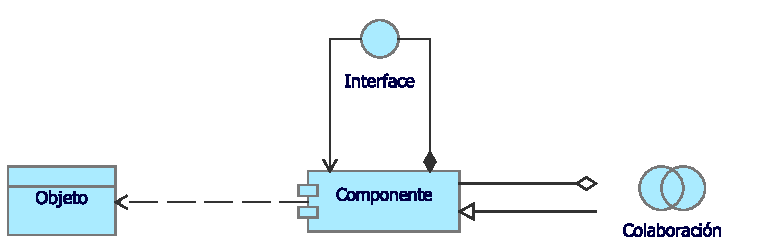
\includegraphics[width=.8\linewidth]{imgs/modelo/EstrAplicacion}
	\caption{Modelo Estructura de Aplicación}
\end{figure}

Una interfaz de aplicación especifica cómo se puede acceder a la funcionalidad de un componente mediante otros elementos. Una interfaz de aplicación expone los servicios de aplicación al entorno. El mismo servicio de aplicación puede estar expuesto a través de diferentes interfaces, y la misma interfaz puede exponer múltiples servicios.
En cierto sentido, una interfaz de aplicación especifica un tipo de contrato que un componente que expone esta interfaz debe cumplir. Esto puede incluir parámetros, protocolos utilizados, condiciones previas y posteriores y formatos de datos.
Una interfaz de aplicación puede formar parte de un componente de la aplicación a través de la composición, lo que significa que estas interfaces son proporcionadas por ese componente, y pueden servir a otros componentes de la aplicación. Una interfaz de aplicación puede asignarse a servicios de aplicación, lo que significa que la interfaz expone estos servicios al entorno. El nombre de una interfaz de aplicación debería ser preferentemente un sustantivo.

\newpage

\subsection{Caso  de Estructura de Aplicación}
\begin{figure}[h!]
	\centering
	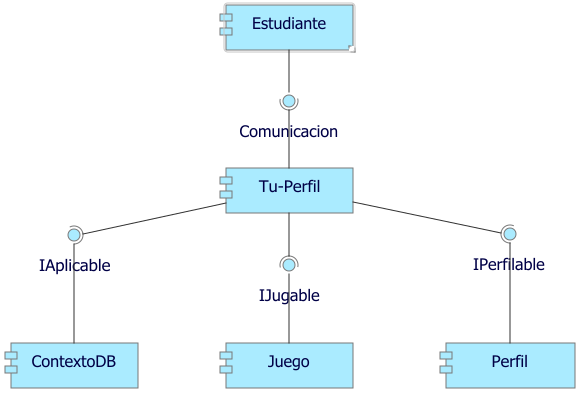
\includegraphics[width=.8\linewidth]{imgs/caso/aplicacion/estructura}
	\caption{Caso Estructura de Aplicación}
\end{figure}

La estructura de aplicación para el producto TU-PERFIL, esta compuesta por cinco componentes incluyendo el mismo, que cumple la función de orquestar a los demás componentes a través de las interfaces provistas para cada uno de los servicios. A saber, cuenta con una interfaz ContextDB, la cual brinda información actualizada desde la base datos, sobre aquellas profesiones con una mayor demanda y ajustadas al contexto local, mediante su interfaz IAplicable. Juego, es otro componente que permite recopilar datos de perfilamiento mediante el concepto de la GAMIFICACIÓN de procesos y conceptos, valiéndose de su interfaz IJugable. Pro otra parte, el componente Perfil realiza un tratamiento de datos para categorizar los datos a disposición, dentro de alguna de las categorías para perfiles através de su interfaz IPerfilable. Pro último, el componente estudiante dispone de una interfaz Comunicación para socializar los resultados obtenidos del proceso de acompañamiento y perfilamiento.

\newpage